\documentclass[12pt]{article}
\usepackage[left=1cm, right=1cm, top=2cm,bottom=1.5cm]{geometry} 

\usepackage[parfill]{parskip}
\usepackage[utf8]{inputenc}
\usepackage[T2A]{fontenc}
\usepackage[russian]{babel}
\usepackage{enumitem}
\usepackage[normalem]{ulem}
\usepackage{amsfonts, amsmath, amsthm, amssymb, mathtools,xcolor}
\usepackage{blkarray}

\usepackage{tabularx}
\usepackage{hhline}

\usepackage{accents}
\usepackage{fancyhdr}
\pagestyle{fancy}
\renewcommand{\headrulewidth}{1.5pt}
\renewcommand{\footrulewidth}{1pt}

\usepackage{graphicx}
\usepackage[figurename=Рис.]{caption}
\usepackage{subcaption}
\usepackage{float}

%%Наименование папки откуда забирать изображения
\graphicspath{ {./images/} }

%%Изменение формата для ввода доказательства
\renewcommand{\proofname}{$\square$  \nopunct}
\renewcommand\qedsymbol{$\blacksquare$}

%%Изменение отступа на таблицах
\addto\captionsrussian{%
	\renewcommand{\proofname}{$\square$ \nopunct}%
}
%% Римские цифры
\newcommand{\RN}[1]{%
	\textup{\uppercase\expandafter{\romannumeral#1}}%
}

%% Для удобства записи
\newcommand{\MR}{\mathbb{R}}
\newcommand{\MC}{\mathbb{C}}
\newcommand{\MQ}{\mathbb{Q}}
\newcommand{\MN}{\mathbb{N}}
\newcommand{\MZ}{\mathbb{Z}}
\newcommand{\MTB}{\mathbb{T}}
\newcommand{\MTI}{\mathbb{I}}
\newcommand{\MI}{\mathrm{I}}
\newcommand{\MCI}{\mathcal{I}}
\newcommand{\MJ}{\mathrm{J}}
\newcommand{\MH}{\mathrm{H}}
\newcommand{\MT}{\mathrm{T}}
\newcommand{\MU}{\mathcal{U}}
\newcommand{\MV}{\mathcal{V}}
\newcommand{\MB}{\mathcal{B}}
\newcommand{\MF}{\mathcal{F}}
\newcommand{\MW}{\mathcal{W}}
\newcommand{\ML}{\mathcal{L}}
\newcommand{\MP}{\mathcal{P}}
\newcommand{\VN}{\varnothing}
\newcommand{\VE}{\varepsilon}

\theoremstyle{definition}
\newtheorem{defn}{Опр:}
\newtheorem{rem}{Rm:}
\newtheorem{prop}{Утв.}
\newtheorem{exrc}{Упр.}
\newtheorem{lemma}{Лемма}
\newtheorem{theorem}{Теорема}
\newtheorem{corollary}{Следствие}

\newenvironment{cusdefn}[1]
{\renewcommand\thedefn{#1}\defn}
{\enddefn}

\DeclareRobustCommand{\divby}{%
	\mathrel{\text{\vbox{\baselineskip.65ex\lineskiplimit0pt\hbox{.}\hbox{.}\hbox{.}}}}%
}
%Короткий минус
\DeclareMathSymbol{\SMN}{\mathbin}{AMSa}{"39}
%Длинная шапка
\newcommand{\overbar}[1]{\mkern 1.5mu\overline{\mkern-1.5mu#1\mkern-1.5mu}\mkern 1.5mu}
%Функция знака
\DeclareMathOperator{\sgn}{sgn}

%Функция ранга
\DeclareMathOperator{\rk}{\text{rk}}

%Обозначение константы
\DeclareMathOperator{\const}{\text{const}}

\DeclareMathOperator{\codim}{\text{codim}}

\DeclareMathOperator*{\dsum}{\displaystyle\sum}
\newcommand{\ddsum}[2]{\displaystyle\sum\limits_{#1}^{#2}}

%Интеграл в большом формате
\DeclareMathOperator{\dint}{\displaystyle\int}
\newcommand{\ddint}[2]{\displaystyle\int\limits_{#1}^{#2}}
\newcommand{\ssum}[1]{\displaystyle \sum\limits_{n=1}^{\infty}{#1}_n}

\newcommand{\smallerrel}[1]{\mathrel{\mathpalette\smallerrelaux{#1}}}
\newcommand{\smallerrelaux}[2]{\raisebox{.1ex}{\scalebox{.75}{$#1#2$}}}

\newcommand{\smallin}{\smallerrel{\in}}
\newcommand{\smallnotin}{\smallerrel{\notin}}

\newcommand*{\medcap}{\mathbin{\scalebox{1.25}{\ensuremath{\cap}}}}%
\newcommand*{\medcup}{\mathbin{\scalebox{1.25}{\ensuremath{\cup}}}}%

\makeatletter
\newcommand{\vast}{\bBigg@{3.5}}
\newcommand{\Vast}{\bBigg@{5}}
\makeatother

%Промежуточное значение для sup\inf, поскольку они имеют разную высоту
\newcommand{\newsup}{\mathop{\smash{\mathrm{sup}}}}
\newcommand{\newinf}{\mathop{\mathrm{inf}\vphantom{\mathrm{sup}}}}

%Скалярное произведение
\newcommand{\inner}[2]{\left\langle #1, #2 \right\rangle }
\newcommand{\linsp}[1]{\left\langle #1 \right\rangle }
\newcommand{\linmer}[2]{\left\langle #1 \vert #2\right\rangle }

%Подпись символов снизу
\newcommand{\ubar}[1]{\underaccent{\bar}{#1}}

%% Шапка для букв сверху
\newcommand{\wte}[1]{\widetilde{#1}}
\newcommand{\wht}[1]{\widehat{#1}}

%%Трансформация Фурье
\newcommand{\fourt}[1]{\mathcal{F}\left(#1\right)}
\newcommand{\ifourt}[1]{\mathcal{F}^{-1}\left(#1\right)}

%%Символ вектора
\newcommand{\vecm}[1]{\overrightarrow{#1\,}}

%%Пространстов матриц
\newcommand{\mat}[2]{\operatorname{Mat}_{#1, #2}}


%%Взятие в скобки, модули и норму
\newcommand{\parfit}[1]{\left( #1 \right)}
\newcommand{\modfit}[1]{\left| #1 \right|}
\newcommand{\sqparfit}[1]{\left\{ #1 \right\}}
\newcommand{\normfit}[1]{\left\| #1 \right\|}

%%Функция для обозначения равномерной сходимости по множеству
\newcommand{\uconv}[1]{\overset{#1}{\rightrightarrows}}
\newcommand{\uconvm}[2]{\overset{#1}{\underset{#2}{\rightrightarrows}}}


%%Функция для обозначения нижнего и верхнего интегралов
\def\upint{\mathchoice%
	{\mkern13mu\overline{\vphantom{\intop}\mkern7mu}\mkern-20mu}%
	{\mkern7mu\overline{\vphantom{\intop}\mkern7mu}\mkern-14mu}%
	{\mkern7mu\overline{\vphantom{\intop}\mkern7mu}\mkern-14mu}%
	{\mkern7mu\overline{\vphantom{\intop}\mkern7mu}\mkern-14mu}%
	\int}
\def\lowint{\mkern3mu\underline{\vphantom{\intop}\mkern7mu}\mkern-10mu\int}

%%След матрицы
\DeclareMathOperator*{\tr}{tr}

\makeatletter
\renewcommand*\env@matrix[1][*\c@MaxMatrixCols c]{%
	\hskip -\arraycolsep
	\let\@ifnextchar\new@ifnextchar
	\array{#1}}
\makeatother

\begin{document}
\lhead{Алгебра-\RN{1}}
\chead{Тимашев Д.А.}
\rhead{Лекция - 3}
\section*{Векторные пространства}
Пусть $V$ - векторное пространство, $S \subseteq V$ - система векторов, выберем $B \subseteq S$- конечная система.

\begin{defn}
	Система векторов $S$ называется \uwave{максимальной линейно независимой} подсистемой, если её нельзя увеличить с тем, чтобы свойство линейной независимости сохранилось.
\end{defn}

\begin{prop}
	Следующие условия эквивалентны:
	\begin{enumerate}[label=(\arabic*)]
		\item $B$ - максимальная линейно независимая подсистема в $S$;
		\item $B$ - линейно независима, и $\forall v \in S$ линейно выражается через $B$;
	\end{enumerate}
\end{prop}
\begin{proof}
	Обозначим векторы в системе $B = \{v_1,\dotsc, v_r\}$.
	
	$(1) \Rightarrow (2)$ Предположим, что $v \in B \Rightarrow  v = v_i = 0{\cdot}v_1 + \dotsc + 1{\cdot}v_i + \dotsc + 0{\cdot}v_r \Rightarrow$ мы получили, что вектор $v$ линейно выражается через систему $B$. Пусть теперь $v \in S\setminus B \Rightarrow B \cup \{v\}$ - линейно зависима $\Rightarrow$ вектор $v$ можно выразить единственным образом через векторы $B$ (по утверждению $9$ с прошлой лекции):
	
	$(2) \Rightarrow (1)$ Пусть $v \in S \setminus B \Rightarrow v$ линейно выражается через $B$ по условию $\Rightarrow$ система $B \cup \{v\}$ - линейно зависима (по свойству $8$ с прошлой лекции) $\Rightarrow B$ - максимальная линейно независимая подсистема.
\end{proof}

\begin{defn}
	Конечная подсистема $B \subseteq S$ удовлетворяющая любому из эквивалентных условий:
	\begin{enumerate}[label=(\arabic*)]
		\item $B$ - максимальная линейно независимая подсистема в $S$;
		\item $B$ - линейно независима, и $\forall v \in S$ линейно выражается через $B$;
	\end{enumerate}
	называется \uwave{базисом} системы векторов $S$.
\end{defn}

\subsection*{Примеры базисов}
Будем считать $S = V$.
\begin{enumerate}[label=(\arabic*)]
	\item $V = \{\text{геом. векторы на прямой}\}$.
	
	\textbf{\uline{Базис}}: $B = \{v\}, \, v \neq 0$ по условию $(2)$, поскольку любой другой вектор имеет вид $\lambda{\cdot}v$.
	\begin{figure}[H]
		\centering
		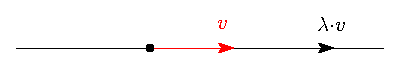
\includegraphics[width=0.35\textwidth]{AL3_1.eps}
		\caption{Базис пространства геометрических векторов на прямой.}
		\label{3_1}
	\end{figure}
	\begin{proof}
		Очевидно по условию $(2)$.
	\end{proof}
	\item $V = \{\text{геом. векторы на плоскости}\}$.
	
	\textbf{\uline{Базис}}: $B = \{v_1, v_2\}, \, v_1,v_2 \neq 0$ и не коллинеарны (не пропорциональны). 
	\begin{proof}
		Любой вектор на плоскости можно спроектировать на прямую на которой находится вектор $v_1$ параллелльно прямой на которой находится $v_2$. Аналогично можно спроектировать $v$ на прямую на которой находится вектор $v_2$ параллельно прямой на которой находится $v_1$. Тогда вектор $v$ будет суммой этих проекций: $\lambda_1 v_1 + \lambda_2 v_2$ и любой вектор на плоскости можно представить в виде линейной комбинации двух неколлинеарных векторов $\Rightarrow$ по  условию $(2)$ это будет базис.
	\end{proof}

	\begin{figure}[H]
		\centering
		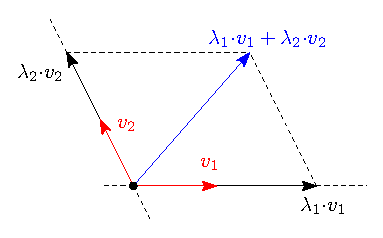
\includegraphics[width=0.35\textwidth]{AL3_2.eps}
		\caption{Базис пространства геометрических векторов на плоскости.}
		\label{3_2}
	\end{figure}

	\item $V = \{\text{геом. векторы в пространстве}\}$.
	
	\textbf{\uline{Базис}}: $B = \{v_1, v_2, v_3\}, \, v_1,v_2, v_3 \neq 0$ и не лежат в одной плоскости.
	\begin{figure}[H]
		\centering
		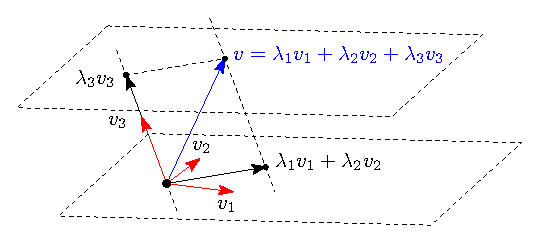
\includegraphics[width=0.55\textwidth]{AL3_3.eps}
		\caption{Базис пространства геометрических векторов в пространстве.}
		\label{3_3}
	\end{figure}
	\begin{proof}
		Спроектируем на плоскость, где лежат векторы $\{v_1,v_2\}$ вектор $v$ параллельно прямой на которой лежит $v_3 \Rightarrow$ получим вектор в плоскости: $\lambda_1 v_1 + \lambda_2 v_2$. С другой стороны, спроектируем вектор $v$ на прямую на которой лежит $v_3$ параллельно плоскости в которой лежат $\{v_1,v_2\} \Rightarrow$ проведем параллельную плоскость через конец вектора $v$ и посмотрим, где она пересечёт прямую на которой лежит вектор $v_3$. 
		
		Таким образом $v = \lambda_1 v_1 + \lambda_2 v_2 + \lambda_3 v_3$. Сами вектора не лежат в одной плоскости $\Rightarrow$ линейно независимы по примеру из прошлой лекции (найдется вектор, который не лежит в плоскости с остальными двумя) $\Rightarrow$ по пункту $(2)$ это базис.
	\end{proof}
	
	\item $V = \MR^n$ - \uwave{арифметическое пространство}.
	
	\textbf{\uline{Базис}}: стандартный базис $B = \{e_1,\dotsc,e_n\}$.
	\begin{proof}
		Докажем линейную независимость $\Rightarrow$ возьмем произвольную линейную комбинацию:
		$$
			\lambda_1 e_1 + \dotsc + \lambda_i e_i + \dotsc + \lambda_n e_n = 
		$$
		$$
			= (\lambda_1, \dotsc, 0, 0 , 0 , \dotsc, 0 ) + \dotsc + (0, \dotsc, 0, \lambda_i , 0 , \dotsc, 0 ) + \dotsc + (0, \dotsc, 0, 0 , 0 , \dotsc, \lambda_n ) =
		$$
		$$
			= (\lambda_1, \dotsc, \lambda_{i-1},\lambda_i, \lambda_{i+1}, \dotsc, \lambda_n) = 0 \Leftrightarrow \lambda_1  = \dotsc = \lambda_i = \dotsc = \lambda_n = 0
		$$
		Проверим, что любой вектор $x \in \MR^n$ выражается через эти вектора:
		$$
			\forall x \in \MR^n, \, x = (x_1 ,\dotsc, x_i, \dotsc, x_n) = x_1 e_1 + \dotsc + x_i e_i + \dotsc + x_n e_n
		$$
		Следовательно, по $(2)$ это базис.
	\end{proof}
\end{enumerate}
\begin{defn}
	\uwave{Стандартным базисом} арифметического пространства $\MR^n$ называется следующая система векторов: $B = \{e_1,\dotsc,e_n\}$, где $e_i = (\underset{1}{0}, \dotsc, \underset{i-1}{0}, \underset{i}{1}, \underset{i+1}{0}, \dotsc, \underset{n}{0})$.
\end{defn}

\subsection*{Свойства базиса}
\begin{prop}
	Пусть $B = \{v_1, \dotsc, v_r\}$ - базис системы векторов $S$, тогда $\forall v\in S,\, \exists! \,$ выражение этого вектора через базисные: 
	$$
		v = \lambda_1 v_1 + \dotsc + \lambda_rv_r
	$$
\end{prop}
\begin{proof}\hfill\\
	\uline{\textbf{Существование}}: следует сразу из условия $(2)$ в определении базиса.
	
	\uline{\textbf{Единственность}}: пусть $ v = \lambda_1 v_1 + \dotsc + \lambda_rv_r = \mu_1 v_1 + \dotsc + \mu_r v_r \Rightarrow$ вычтем одно из другого:
	$$
		0 = (\lambda_1 - \mu_1)v_1 + \dotsc + (\lambda_r - \mu_r)v_r \Rightarrow \lambda_1 - \mu_1 = \dotsc = \lambda_r - \mu_r = 0
	$$
	где последнее верно в силу линейной независимости базиса, тогда:
	$$
		\lambda_i =  \mu_i , \, \forall i = \overline{1,r}
	$$
\end{proof}
\begin{defn}
	Пусть $B = \{v_1, \dotsc, v_r\}$ - базис системы векторов $S$, $\forall v \in S$, скаляры $\lambda_1,\dotsc, \lambda_r$ в его разложении: 
	$$
		v = \lambda_1 v_1 + \dotsc +  \lambda_r v_r
	$$
	называются \uwave{координатами} векотора $v$ в базисе $B$.
\end{defn}
\begin{rem}
	Каждый вектор задается своими координатами в каком-то базисе.
\end{rem}

\textbf{Пример}: Координаты вектора $x = (x_1,\dotsc,x_n) \in \MR^n$ в стандартном базисе:
$$
	x = (x_1,\dotsc,x_n) = x_1 e_1  + \dotsc + x_n e_n
$$
То есть, координаты это числа $x_1, \dotsc, x_n$.

Возникает вопрос, а всякая ли система векторов в векторном пространстве имеет базис. Покажем, что это верно для систем векторов в арифметическом пространсте.
\begin{prop}
	\hfill
	\begin{enumerate}[label=\arabic*)]
		\item Любая система векторов $S \subseteq \MR^n$ обладает базисом;
		\item Во всех базисах системы $S$ одинаковое количество векторов, причем $\leq n$, если  $S \subseteq \MR^n$;
	\end{enumerate}
\end{prop}
\begin{proof}\hfill
	\begin{enumerate}[label=\arabic*)]
		\item \uline{\textbf{Построение базиса системы}} $S$: 
		
		Если $S = \VN$ или $S = \{0\}$, то базисных векторов вообще нет, поскольку нет линейно независимых подсистем, кроме пустого множества $\Rightarrow B = \VN$.
		
		Если $S \neq \VN$, возьмем $v_1 \in S, \, v_1 \neq 0 \Rightarrow \{v_1\}$ - линейно независима и дальше возможны два случа: либо она не максимальна, либо максимальна и это базис. Если она не максимальна, то расширим её, добавив ещё один вектор, до линейно назвисимой системы $\{v_1,v_2\} \subseteq S$. И так далее. 
		
		Получим возрастающую цепочку линейно независимых подсистем:
		$$
			\{v_1\} \subset \{v_1,v_2\} \subset \dotsc \subset \{v_1 ,\dotsc, v_k\} \subset \dotsc \subseteq S \subseteq \MR^n
		$$
		Из последнего следует, что любая из этих систем $\{v_1, \dotsc, v_k\}$ линейно выражается через $\{e_1, \dotsc, e_n\}$, но поскольку система $\{v_1,\dotsc,v_k\}$ линейно независима, то по основной лемме о линейной зависимости $k \leq n \Rightarrow$ цепочка вложений - конечна: $\exists \, r \leq n \colon B = \{v_1, \dotsc, v_r\}$ - будет максимальной линейно независимой подсистемой в системе $S \Rightarrow B$ - базис по $(1)$ определения.
 		
 		\item Пусть у нас есть другой базис $B' =\{w_1,\dotsc, w_s\} \Rightarrow$ он линейно выражается через $B$, поскольку через $B$ выражаются все векторы системы $\Rightarrow$ по основной лемме о линейной зависимости $s \leq r$. 
 		
 		Аналогично, $B$ выражается через $B'$, потому что $B'$ это тоже базис и по той же самой основной лемме о линейной зависимости будет верно: $r \leq s \Rightarrow s = r$.
 	\end{enumerate}
\end{proof}
\begin{corollary}
	Любое линейно независимое подмножество $v_1, \dotsc, v_s$ в $S$ можно дополнить до базиса.
\end{corollary}

\begin{defn}
	\uwave{Ранг системы} векторов $S$ это количество векторов в любом её базисе.
	
	\uline{\textbf{Обозначение}}: $\rk{S}$.
\end{defn}
\begin{rem}
	Другими словами ранг системы векторов равен максимальному количеству линейно независимых векторов, которые можно выбрать из этой системы.
\end{rem}
В случае, когда $S = V$ вместо ранга используют размерность (по сути это одно и то же).
\begin{defn}
	\uwave{Размерность} векторного пространства $V$ это количество векторов в любом его базисе. 
	
	\uline{\textbf{Обозначение}}: $\dim{V}$.
\end{defn}
\begin{defn}
	Векторные пространства, обладающие конечным базисом называются \uwave{конечномерными}. В противном случае, они называются \uwave{бесконечномерными}.
\end{defn}

\subsection*{Примеры размерности векторных пространства}
\begin{enumerate}[label=\arabic*)]
	\item $V = \{\text{геом. векторы на прямой}\} \Rightarrow B = \{v_1\} \Rightarrow \dim{V} = |B| = 1$;
	\item $V = \{\text{геом. векторы на плоскости}\}\Rightarrow B = \{v_1, v_2\} \Rightarrow \dim{V} = |B| = 2$;
	\item $V = \{\text{геом. векторы в пространстве}\}\Rightarrow B = \{v_1, v_2, v_3\} \Rightarrow \dim{V} = |B| = 3$;
	\item $V = \MR^n \Rightarrow$ стандартный базис из $n$ векторов: $B = \{e_1,\dotsc,e_n\} \Rightarrow \dim{V} = |B| = n$;
\end{enumerate}

\begin{prop}
	Пусть $V$ - конечномерное векторное пространство, $\dim{V} = n$ с базисом $\{v_1,\dotsc, v_n\}$. Тогда возникает взаимнооднозначное соответствие: $V \leftrightarrow \MR^n$, которое сопоставляет каждому вектору $v \in V$ строчку его координат $(\lambda_1,\dotsc,\lambda_n)$.
\end{prop}
\begin{proof}
	По свойству базиса верно: 
	$$
		\forall v \in V, \, \exists ! \lambda_1, \dotsc, \lambda_n \in \MR \colon v = \lambda_1 v_1 + \dotsc + \lambda_n v_n
	$$
	Предъявим соответствие: $\varphi \colon V \to \MR^n, \, \varphi(v) = (\lambda_1, \dotsc, \lambda_n)$. Оно очевидно инъективно и сюръективно в силу существования и единственности разложения $v$ по базису $\Rightarrow$ оно взаимнооднозначное.
\end{proof}
\begin{rem}
	Такое взаимнооднозначное соответствие позволяет отождествить $V$ с $\MR^n$.
\end{rem}
Далее мы будем рассматривать в основном арифметические векторные пространства, но с помощью этого отождествления можно будет перенести всё что докажем дословно на любое конечномерное пространство без изменения.


\subsection*{Свойства ранга системы векторов}

\begin{prop}
	Если $S \subseteq S'$, то $\rk{S} \leq \rk{S'}$.
\end{prop}
\begin{proof}
	Пусть $B$ - базис системы $S$, тогда $B$ - линейно независимая подсистема в $S \Rightarrow$ и в системе $S'$ она также будет линейно независимой (просто по определению) $\Rightarrow B \subseteq B'$, где $B'$ - базис системы $S'$. То есть мы можем расширить $B$ до базиса системы $S'$ по построению базиса из утверждения $3 \Rightarrow$ число векторов в $B$ не больше, чем в $B' \Rightarrow |B| \leq |B'| \Rightarrow \rk{S} \leq \rk{S'}$. 
\end{proof}

\begin{prop}
	Если система $S$ линейно выражается через $S'$ (то есть  $\forall s \in S$ является линейной комбинацией векторов из $S'$), то $\rk{S} \leq \rk{S'}$.
\end{prop}
\begin{proof}
	Пусть $B$ - базис в $S$, $B'$ - базис в $S'$, тогда по условию $B$ линейно выражается через $S'$, которая выражается через $B' \Rightarrow B$ линейно выражается через $B' \Rightarrow$  поскольку $B$ - линейно независимая система, то по ОЛЛЗ верно, что: $|B| \leq |B'| \Rightarrow \rk{B} \leq \rk{B'}$.
\end{proof}

\begin{defn}
	Системы векторов $S$ и $S'$ называются \uwave{линейно эквивалентными}, если они линейно выражаются друг через друга.
\end{defn}
\begin{prop}
	Пусть системы векторов $S$ и $S'$ линейно выражаются друг через друга, то есть линейно эквивалентны, тогда их ранги совпадают: $\rk{S} = \rk{S'}$.
\end{prop}
\begin{proof}
	Из предыдущего утверждения, у нас будет два неравенства: $\rk{B} \leq \rk{B'}$ и $\rk{B'} \leq \rk{B}$.
\end{proof}
\begin{prop}
	Элементарные преобразования не изменяют ранг системы векторов.
\end{prop}
\begin{proof}
	Если $v'_1, \dotsc, v'_n$ получены из $v_1, \dotsc, v_n$ цепочкой элементарных преобразований,то $v'_1, \dotsc, v'_n$ это линейные комбинации $v_1, \dotsc, v_n$. Применяя обратно ЭП выразим $v_1, \dotsc, v_n$ через $v'_1, \dotsc, v'_n \Rightarrow$ системы эквивалентны $\Rightarrow$ у эквивалентных систем ранги совпадают
\end{proof}

\section*{Ранг матрицы}
\begin{defn}
	\uwave{Матрица порядка} $m \times n$ - это прямоугольная таблица, заполненная числами, состоящая из $m$ строк и $n$ столбцов.
\end{defn}
Пусть $A$ - матрица размера $m\times n$:
$$
	A = 
	\begin{pmatrix}
		a_{11} & \dotsc & a_{1n}\\
		a_{21} & \dotsc & a_{2n}\\
		\vdots & \ddots & \vdots \\
		a_{m1} & \dotsc & a_{mn}
	\end{pmatrix}
$$
Обозначим её строки $A_1, A_2, \dotsc, A_m \in \MR^n$ и каждая из строчек это строка длины $n$, то есть это вектор из арифметического $n$-мерного пространства. Столбцы матрицы обозначим $A^{(1)}, \dotsc, A^{(n)} \in \MR^m$ - векторы из арифметического $m$-мерного пространства.

\begin{defn}
	\uwave{Горизонтальным рангом} матрицы $A$ назовем ранг системы её строк: $\rk{\left\{A_1, \dotsc, A_m\right\}}$.\\
	\uline{\textbf{Обозначение}}: $r_h(A)$.
\end{defn}
\begin{defn}
	\uwave{Вертикальным рангом} матрицы $A$ назовем ранг системы её столбцов: $\rk{\left\{A^{(1)}, \dotsc, A^{(n)}\right\}}$.\\
	\uline{\textbf{Обозначение}}: $r_v(A)$.
\end{defn}
Приведем матрицу $A$ к ступенчатом виду ЭП строк и получим матрицу $A^*$.
\begin{defn}
	\uwave{Ступенчатым рангом} матрицы $A^*$ назовем количество её ненулевых строк.\\
	\uline{\textbf{Обозначение}}: $r_{e}(A^*)$, где $e$ - от echelon.
\end{defn}

\begin{defn}
	\uwave{Транспонированная матрица} $A^T$ это матрица, которая получается из исходной матрицы отражением всех элементов относительно диагонали идущей из верхнего левого угла вниз под $45^\circ$.
\end{defn}
$$
	A = 
	\begin{pmatrix}
		a_{11} & a_{12} & \dotsc & a_{1n}\\
		a_{21} & a_{22} & \dotsc & a_{2n}\\
		\vdots & \vdots & \ddots & \vdots \\
		a_{m1} & a_{m2} & \dotsc & a_{mn}
	\end{pmatrix} \Rightarrow A^T =
	\begin{pmatrix}
		a_{11} & a_{21} & \dotsc & a_{m1}\\
		a_{12} & a_{22} & \dotsc & a_{m2}\\
		\vdots & \vdots & \ddots & \vdots \\
		a_{1n} & a_{2n} & \dotsc & a_{mn}
	\end{pmatrix}
$$
Транспонированная матрица будет иметь размер $n \times m$ и её элементы будут равны: $a_{ij}^T = a_{ji}$.\\
Строки транспонированной матрицы это столбцы исходной матрицы: $A_i^T = A^{(i)}, \, i =\overline{1,n}$.\\
Столбцы транспонированной матрицы это строки исходной матрицы: $\left(A^T\right)^{(j)} = A_j, \, j =\overline{1,m}$.
\begin{prop}
	$r_{h}(A^T) = r_v(A), \, r_v\left(A^T\right) = r_h(A)$.
\end{prop}
\begin{proof}
	Очевидно, поскольку:
	$$
		r_h\left(A^T\right) = \rk{\left\{A_1^T, \dotsc, A_n^T\right\}} = \rk{\left\{A^{(1)}, \dotsc, A^{(n)}\right\}} = r_v(A)
	$$
	$$
		r_v\left(A^T\right) = \rk{\left\{\left(A^T\right)^{(1)}, \dotsc, \left(A^T\right)^{(m)}\right\}} = \rk{\left\{A_1, \dotsc, A_m\right\}}  = r_h(A)
	$$
\end{proof}
\begin{theorem}
	$r_h(A) = r_v(A) = r_{e}(A^*)$.
\end{theorem}
\begin{proof}
	Докажем теорему в несколько шагов.
	\begin{enumerate}[label=\arabic*)]
		\item Докажем, что $r_h(A)$ не меняется при ЭП строк матрицы $A$. 
		
		Пусть мы применили к $A$ ЭП строк и получили матрицу $A'$. По устройству ЭП строк, получаемые строки являются линейными комбинациями строк исходной матрицы $\Rightarrow \{A'_1,\dotsc, A'_m\}$ линейно выражается через $\{A_1,\dotsc, A_m\}$ и наоборот, поскольку есть обратные ЭП строк, которые могут вернуть $A'$ в первоначальный вид. То есть эти две системы строк эквивалентны $\Rightarrow$ у линейно эквивалентных систем ранги совпадают $\Rightarrow r_h(A) = r_h(A')$ по утверждению $7$;
		
		\item Вертикальный ранг $r_v(A)$ не меняется при ЭП строк матрицы $A$.
		
		Рассмотрим ОСЛУ следующего вида:
		$$
			\left\{
			\begin{array}{ccccccc}
				a_{11}x_1 & + & \dotsc & + & a_{1n}x_n & = & 0 \\
				\vdots & \vdots &  \ddots & \vdots & \vdots & \vdots & \vdots \\ 
				a_{m1}x_1 & + & \dotsc & + & a_{mn}x_n & = & 0 
			\end{array}
			\right.
		$$
		Набор чисел $(\lambda_1, \dotsc, \lambda_n)$ является решением этой ОСЛУ $\Leftrightarrow$ при подстановке в каждое из этих уравнений он даёт верное равенство:
		$$
			\forall i = \overline{1,m}, \, a_{i1}\lambda_1 + \dotsc + a_{in}\lambda_n = 0 \Leftrightarrow A^{(1)}{\cdot}\lambda_1 + \dotsc + A^{(2)}{\cdot}\lambda_n = 0
		$$
		Таким образом, ненулевые решение ОСЛУ это тоже самое, что и линейные зависимости между столбцами $A^{(1)}, \dotsc, A^{(n)}$. При ЭП строк матрицы $A$ мы получим матрицу $A'$, но множество решений ОСЛУ не изменится (утверждение $1$, лекция $1$) $\Rightarrow$ линейные зависимости между столбцами новой матрицы: $(A')^{(1)}, \dotsc, (A')^{(n)}$ такие же, как между столбцами исходной матрицы $A^{(1)}, \dotsc, A^{(n)}$. 
		
		В частности, если $\left\{A^{(j_1)}, \dotsc, A^{(j_r)}\right\}$ это базис системы столбцов $A$, то тогда $\left\{(A')^{(j_1)}, \dotsc, (A')^{(j_r)}\right\}$ это уже базис системы столбцов $A'$. Если исходная система была линейно независимой, то и новая будет (поскольку линейные зависимости сохранятся). Если исходная была максимальной, то и новая будет, а иначе можно добавить к новой ещё один вектор и сохранить линейную независимость $\Rightarrow$ и к исходной можно будет добавить столбец $\Rightarrow$ противоречие и максимальность сохраняется. Таким образом, $r_v(A) = r_v(A') = r$ - число элементов в базисе.
		
		\item Горизонтальный и вертикальные ранги сохраняются и при ЭП столбцов $A$.
		
		ЭП столбцов $A \Leftrightarrow $ ЭП строк $A^T$, а мы знаем, что $r_{h}(A^T) = r_v(A), \, r_v\left(A^T\right) = r_h(A)$. 
		
		\item Приведем матрицу $A$ ЭП строк к улучшенному ступенчатому виду $A^*$. Обозначим столбцы с лидерами строк: $j_1, \dotsc, j_r$.
		$$
			\begin{blockarray}{ccccccccccccc}
				\begin{block}{c(cccccccccc|c)c}			
					& 0 & \dotsc & 0 & 1 & * & 0 & \dotsc & 0 & \dotsc & * &* & 1\\ 
					& 0 & \dotsc & 0 & 0 & 0 & 1 & \dotsc & 0 &\dotsc & * & * & 2\\  
					& \vdots & \ddots & \vdots & \vdots & \vdots & \vdots & \ddots & \vdots & \ddots & \vdots &\vdots & \vdots\\ 
					A^{*} =  & 0 & \dotsc & 0 & 0 & 0 & 0 & \dotsc &  1 & \dotsc & * & * & r\\ 
					&0 & \dotsc & 0 & 0 & 0 & 0 &\dotsc &  0 & \dotsc & 0 & 0 & r+1 \\  
					&\vdots & \ddots & \vdots & \vdots & \vdots & \vdots &\ddots & \vdots & \ddots & \vdots & \vdots & \vdots\\  
					&0 & \dotsc & 0 & 0 & 0 & 0 &\dotsc &  0 & \dotsc & 0 & 0 & m\\
				\end{block}
			& &  &  & j_1 &  & j_2 &\dotsc &  j_r &  &  & & 
		\end{blockarray}
		$$
		Ступенчатый ранг матрицы: $A^* \colon r = r_e{(A^*)}$, поскольку у нас $r$ ненулевых строк в $A^*$. Используя ЭП$2$ столбцов, переставим столбцы с лидерами строк в начало:
		$$
			\begin{blockarray}{cccccccc}
				\begin{block}{(cccc|ccc)c}
					1 & 0 & \dotsc & 0 & * & \dotsc & * & 1\\
					0 & 1 & \dotsc & 0 & * & \dotsc & * & 2\\
					\vdots & \vdots & \ddots & \vdots & \vdots & \ddots & \vdots & \vdots\\
					0 & 0 & \dotsc & 1 & * & \dotsc & * & r\\ \cline{1-7}
					0 & 0 & \dotsc & 0 & 0 & \dotsc & 0 & r+ 1\\
					\vdots & \vdots & \ddots & \vdots & \vdots & \ddots & \vdots & \vdots\\
					0 & 0 & \dotsc & 0 & 0 & \dotsc & 0 & m\\
				\end{block}
				1 & 2 & \dotsc & r & r+1 & \dotsc & n & 
			\end{blockarray}
		$$
		Используя ЭП$2$ столбцов, будем вычитать первые $r$ столбцов из остальных столбцов так, чтобы обнулить всё что правее первых $r$ столбцов. Получим матрицу вида:
		$$
			A^{**} = \begin{blockarray}{cccccccc}
				\begin{block}{(cccc|ccc)c}
					1 & 0 & \dotsc & 0 & 0 & \dotsc & 0 & 1\\
					0 & 1 & \dotsc & 0 & 0 & \dotsc & 0 & 2\\
					\vdots & \vdots & \ddots & \vdots & \vdots & \ddots & \vdots & \vdots\\
					0 & 0 & \dotsc & 1 & 0 & \dotsc & 0 & r\\ \cline{1-7}
					0 & 0 & \dotsc & 0 & 0 & \dotsc & 0 & r+ 1\\
					\vdots & \vdots & \ddots & \vdots & \vdots & \ddots & \vdots & \vdots\\
					0 & 0 & \dotsc & 0 & 0 & \dotsc & 0 & m\\
				\end{block}
				1 & 2 & \dotsc & r & r+1 & \dotsc & n & 
			\end{blockarray}
		$$
		При ЭП строк и столбцов матрицы, горизонтальный ранг матрицы не меняется, поэтому:
		$$
			r_h(A) = r_h(A^{**})
		$$
		Базисом системы строк $A^{**}$ являются первые $r$ строк, поскольку: 
		$$
			\forall i = \overline{1,r}, \, A_i^{**} = e_i, \quad \forall i > r, \, A_i^{**} = 0 \Rightarrow \{A_1^{**}, \dotsc, A_r^{**}\} = \{e_1,\dotsc, e_r\} 
		$$
		Следовательно, горизонтальный ранг матрицы $A^{**}$ равен $r$. Абсолютно аналогично:
		$$
			r_v(A) = r_v{(A^{**})} = r
		$$
		Более того, $r_e{(A^*)} = r$, то есть получаем требуемое: $r_h(A) = r_v(A) = r_e(A^*) = r$.
	\end{enumerate}
\end{proof}

\begin{defn}
	\uwave{Рангом матрицы} $A$ называется число $\rk(A) = r_h(A) = r_v(A) = r_{e}(A^*)$.
\end{defn}

\subsection*{Свойства ранга матрицы}
\begin{prop}
	$\rk{A} \leq \min{\{m,n\}}$.
\end{prop}
\begin{proof}
	Горизонтальный ранг матрицы это ранг системы строк, то есть количество векторов в базисе системы строк, но всего строк $m$ штук, а в базисе $\leq m\Rightarrow \rk{A} = r_h(A) \leq m$. Абсолютно аналогичный результат для столбцов: $\rk{A} = r_v(A) \leq n \Rightarrow \rk{A} \leq \min{\{m,n\}}$.
\end{proof}
\begin{prop}
	$\rk{A}$ не меняется при ЭП строк и столбцов этой матрицы.
\end{prop}
\begin{proof}
	Видели при доказательстве теоремы $1$. 
\end{proof}
\begin{prop}
	$\rk{A}$ не меняется при транспонировании: $\rk{A} = \rk{A^T}$.
\end{prop}
\begin{proof}
	$\rk{A} = r_h(A) = r_v(A) = r_v(A^T) = r_h(A^T) = \rk{A^T}$.
\end{proof}

\end{document}